\documentclass[12pt]{article}
\usepackage[a4paper, margin=0.7in]{geometry}
\usepackage{lipsum}
\usepackage{color}   %May be necessary if you want to color links
\usepackage{hyperref}
\usepackage{graphicx}
\usepackage{pdflscape}
\usepackage{rotating}
\usepackage[table]{xcolor}
\usepackage{minted}
\usemintedstyle{vs}
\usepackage{hhline}
\setlength{\tabcolsep}{18pt}
\renewcommand{\arraystretch}{1.5}
\renewcommand{\contentsname}{Indice}
\begin{document}
\title{%
  Esercitazione 2 \\
  \large Realizzazione di una rete WLAN}
\date{}
\author{Leonardo Geusa 4N}
\setcounter{section}{-1}
\maketitle

\centering
\textit{Una azienda di video giochi ha i propri uffici distribuiti su un piano di un edificio. Sono presenti:}

\begin{center}
\begin{minipage}{0.5\textwidth}
\begin{itemize}

\item \textit{la reception con 3 pc e una stampante}
\item \textit{la sala server con due server}
\item \textit{due uffici con 2 pc e una stampante in ciascuno ufficio collegati attraverso in modalità wireless.}
\end{itemize}
\end{minipage}
\end{center}

\textit{Progettare la relativa rete sapendo che l’indirizzo di rete assegnato è 192.X.Y.0/24 dove X è il giorno della
vostra nascita e Y il mese.}

\vspace{30pt}

\tableofcontents

\raggedright

\section{Ipotesi aggiuntive}
\hspace{24pt} Si presuppone che l'azienda abbia bisogno di un accesso ad internet. La rete più adatta per questo progetto è una rete WLAN\footnote{Wireless Local Area Network} con una trasmissione di tipo broadcast e con una topologia a stella estesa. Saranno quindi necessari un router, degli switch e degli AP\footnote{Access Point}.

\section{Analisi della struttura e delle esigenze dell'azienda}

Secondo le informazioni ricevute, l'azienda è costituita da 4 locali:
\begin{itemize}
\item un locale che ospita due server
\item un ufficio per la reception con tre postazioni e una stampante
\item due uffici ognuno con due postazioni una stampante collegati via wireless ad un AP
\end{itemize}
Sono necessari quindi 2 server, 7 postazioni di cui 4 con scheda di rete wireless e 3 stampanti di cui 2 con scheda di rete wireless. Di seguito la rappresentazione grafica dell'azienda. \\
\vspace{40pt}
\begin{figure}[!h]
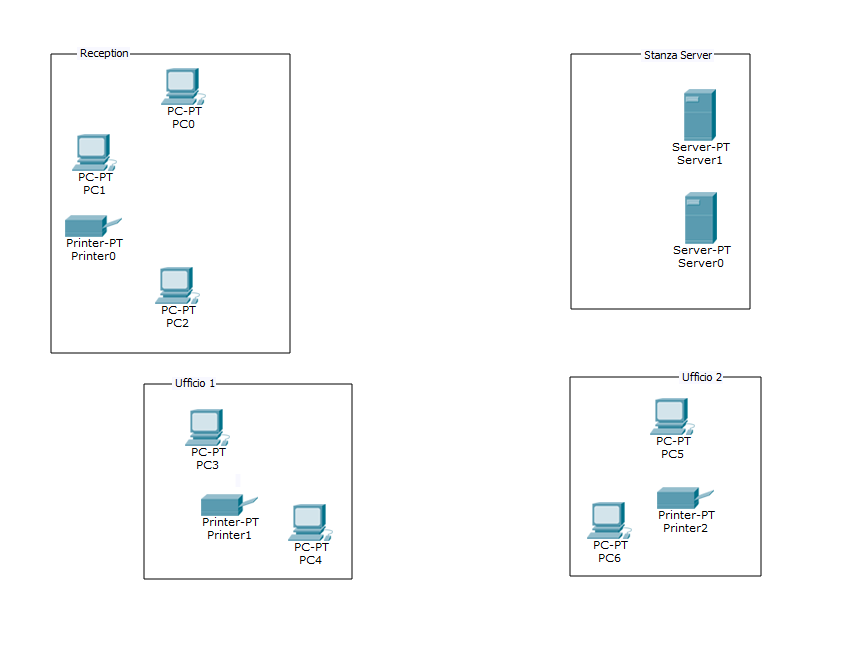
\includegraphics[scale=0.81]{analisi_strutturale}
\label{fig:as1}
\end{figure}
\vspace{40pt}
La rete deve essere efficiente e scalabile, perciò si ha bisogno di cavi e nodi di commutazione che possano soddisfare al massimo queste due richieste.

\section{La classificazione delle reti}
\hspace{24pt}Per questo progetto è più opportuno utilizzare una rete WLAN, dato che la grandezza della rete non deve superare quella di un edificio.

\section{Analisi della topologia fisica e logica}
\hspace{24pt}La topologia fisica che verrà applicata sarà a stella estesa. Questa topologia collega tra loro più reti a stella. Una rete a stella prevede che ciascuno dei nodi sia collegato a un nodo di commutazione centrale, chiamato Punto Stella (di solito uno switch, in questo caso anche AP). È una rete che garantisce una grande tolleranza ai guasti, flessibilità e scalabilità. Tuttavia, se il centro stella è difettoso, questo compromette l'intera rete.\\
\hspace{24pt}La topologia logica che si andrà ad applicare sarà di tipo broadcast, ossia ogni nodo invia i dati mediante una scheda di rete a tutti gli altri nodi.

\section{Analisi degli apparati di rete e mezzi trasmissivi}
Per quanto riguarda gli apparati di rete si andranno ad utilizzare schede di rete (wireless e non), router, AP e switch.\\ \hspace{24pt}La scheda di rete è un dispositivo elettronico installato all'interno di un host che permette il collegamento tra l'host e il cavo, che collega i vari nodi. Una scheda di rete può essere wireless, ossia non ha bisogno di un collegamento fisico via cavo, bensì comunica con l'AP tramite onde radio (etere).\\
\hspace{24pt}Il router è un dispositivo che permette la connessione tra due reti, in particolare una rete LAN e Internet.\\
\hspace{24pt}Lo switch è un dispositivo che collega insieme altri dispositivi. Lo switch, rispetto all'hub, gestisce in modo più efficiente il trasporto dei dati perché inoltra il pacchetto ricevuto soltanto al destinatario.\\
\hspace{24pt}L'AP è un particolare tipo di switch che permette di collegare dispositivi possedenti una scheda di rete wireless, onde evitare di utilizzare troppi cavi. Un AP può essere pubblico o protetto. Se è pubblico non ha bisogno di una chiave d'accesso, se è protetto allora può utilizzare diversi sistemi di sicurezza. Il sistema WEP\footnote{Wired Equivalent Privacy, parte dello standard IEEE 802.11. Questo sistema di crittografia delle reti Wi-Fi fu introdotto per evitare il furto dei dati wireless da parte degli hacker.} prevede la presenza di una chiave per connettersi all'AP. I dati verranno criptati tramite questa chiave, in modo da renderli leggibili soltanto da chi è in possesso della chiave. Un'altro sistema di crittografia è quello di WPA/WPA2\footnote{Wi-Fi Protected Access}, più moderno e più sicuro del WEP.

\newpage

\section{Piano di indirizzamento}
\hspace{24pt}Si procede alla stesura del piano di indirizzamento. L'indirizzo di rete sarà 192.14.10.0/24, l'indirizzo di broadcast sarà 192.14.10.255, la subnet mask sarà 255.255.255.0 e il default gateway sarà 192.14.10.1. Di seguito la tabella con gli indirizzi IP degli host.\\
\vspace{20pt}
\begin{center}
\begin{tabular}{| c | c |}
	\hline
	Hostname & Indirizzo IP \\
	\hline
	Server0 & 192.14.10.4 \\ 
	\hline
	Server1 & 192.14.10.5 \\
	\hline
	PC0 & 192.14.10.6 \\
	\hline
	PC1 & 192.14.10.7 \\
	\hline
	PC2 & 192.14.10.9 \\
	\hline
	PC3 & 192.14.10.10 \\
	\hline
	PC4 & 192.14.10.12 \\
	\hline
	PC5 & 192.14.10.13 \\
	\hline
	PC6 & 192.14.10.15 \\
	\hline
	Printer0 & 192.14.10.8 \\
	\hline
	Printer1 & 192.14.10.11 \\
	\hline
	Printer2 & 192.14.10.14 \\
	\hline
\end{tabular}
\end{center}
\vspace{20pt}

\section{Progettazione della rete}
\hspace{24pt}Per la realizzazione di questa rete è necessario che i server e le postazioni e le stampanti della reception abbiano una scheda di rete di 1 GBit/s. Le postazioni e le stampanti degli uffici, invece, hanno bisogno di una scheda di rete wireless, in particolare si andrà ad utilizzare una scheda \mintinline{batch}{WMP300N}, la quale dota il computer di un'interfaccia di rete che lavora a 2.4GHz. Per sfruttare al massimo le schede di rete è necessario che anche gli switch abbiano porte da 1 GBit/s e che l'AP lavori a 2.4GHz. Si ha infine bisogno dei cavi, in questo caso UTP\footnote{Unshielded Twisted Pair} di 1 GBit/s di categoria 6. Tenendo sempre in considerazione la scalabilità e la flessibilità della rete, si ha quindi bisogno dei seguenti dispositivi di rete:\\
\begin{itemize}
	\item 4 switch: uno da 4 porte per la stanza server, due da 8 porte per il centro stella e la reception.
	\item 1 AP, per la connessione wireless dei due uffici.
	\item 1 router, per la connessione a Internet
	\item 10 cavi UTP: 3 per le connessioni computer - switch, 1 per la connessione stampante - switch, 2 per le connessioni server - switch, 2 per le connessioni switch - centro stella, 1 per la connessione AP - centro stella e uno per la connessione centro stella - router.
\end{itemize}
Di seguito la rappresentazione grafica della rete.
\vspace{30pt}
\begin{figure}[!h]
	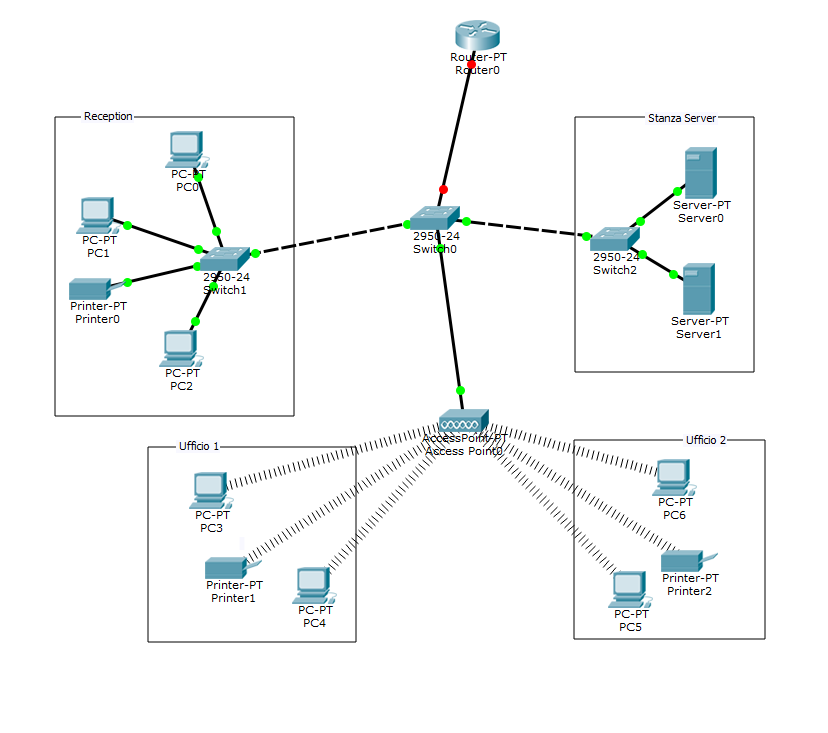
\includegraphics[scale=0.81]{progettazione_rete}
	\label{fig:pr1}
\end{figure}

\section{Configurazione dell'Access Point}
\hspace{24pt}Per questa rete si andrà ad utilizzare un AP con crittografia WEP. L'SSID dell'Access Point è \mintinline{Batch}{AP-Uffici} e la password utilizzata è \mintinline{Batch}{3759173743}. Il canale utilizzato per la trasmissione del segnale (frequenza 2.4GHz) è il 6. In ogni dispositivo negli uffici bisogna configurare la connessione WLAN. Per fare ciò si montano le schede di rete wireless a 2.4GHz e nelle impostazioni di rete si sceglie la modalità WEP e si digita l'SSID e la chiave d'accesso dell'AP.

\newpage

\input{test_connettività}

\vspace{100pt}
Il codice sorgente di questo pdf si trova \href{https://github.com/Leoooog/Esercitazione2}{\textcolor{blue}{qui}}

\end{document}